\documentclass[tikz,border=10pt]{standalone}
\usepackage{tikz}
\usepackage{verbatim}
\usepackage{amsmath,unicode-math}
\begin{document}
	\usetikzlibrary{arrows,positioning} 
	\tikzset{
		%Define standard arrow tip
		>=stealth',
		% Define arrow style
		pil/.style={
			->,
			thick,
			shorten <=2pt,
			shorten >=2pt,}
	}
	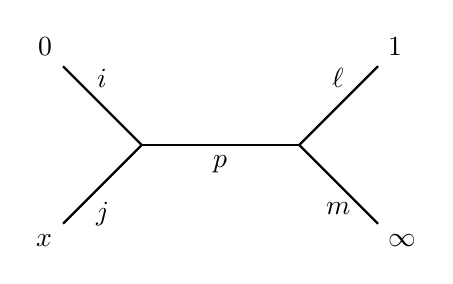
\begin{tikzpicture}
    \draw[thick] (0,0)--(2,0);
    \draw (1,0)node[anchor = north]{$p$};
    \draw[thick] (0,0)--(-1,1) node[anchor = south east]{$0$};
    \draw[thick] (0,0)--(-1,-1) node[anchor = north east]{$x$};
    \draw[thick] (2,0)--(3,1) node[anchor = south west]{$1$};
    \draw[thick] (2,0)--(3,-1) node[anchor = north west]{$\infty$};
    \draw (-0.5,0.6) node[anchor = south]{$i$};
    \draw (-0.5,-0.6) node[anchor = north]{$j$};
    \draw (2.5,0.6) node[anchor = south]{$\ell$};
    \draw (2.5, -0.6) node[anchor = north]{$m$};
\end{tikzpicture}
\end{document}